
\chapter{Sobre o Desenvolvimento}
\label{cap:development}
\minitoc

\intro{Neste capítulo encontram-se reflexões spbre decisões de projeto que foram tomadas e uma reflexão
sobre cada uma. A ideia é que, ao terminar este capítulo, que se possa agrugar as reflexões em temas, de
forma que o conteúdo fique bem organizado. Pode ser que o capítulo ganhe uma feição de página de perguntas
e respostas, e isso é proposital.}

\section{Arquitetura de projeto}\label{sec:arquitetura}

\subsection{Por que as ferramentas descritas foram utilizadas ao invés de outras similares?}
\label{subsec:ferramentas}

No caso do back-end, o Ruby on Rails fora utilizado por alguns motivos. O primeiro, e mais importante é a
continuidade. Como é de conhecimento entre aqueles com maior participação no projeto, o DELPo já foi
desenvolvido em PHP, algumas partes em Pearl, depois Django, e agora em Rails. Muita migração já aconteceu,
e outra estaria praticamente fora de cogitação.

Outro motivo é o fato de que a fluência do aluno em Rails é infinitamente maior em Ruby que Python. Além do
mais, não é só o desenvolvimento que importa: os testes são cruciais, e não há uma ferramenta de testes com
que o aluno esteja perfeitamente familiarizado. Eu precisaria passar por outra curva de aprendizado que, pequena
ou grande, representaria um tempo perdido para essa aplicação em específico.

A fluência e experiência no uso de RSpec também foram fatores determinantes na escolha desta ferramenta. A
escolha do Vue e Nuxt.js também se deve a esses fatores.

Não há muito que se possa falar sobre Angular.js, dado que pouco conheço da ferramenta. Aprender sobre a
ferramenta enquanto a aplicação é feita parece uma ideia pouco sábia a nível estratégico. O aluno responsável
por este trabalho conhece um pouco mais sobre React.js, e isso já é suficiente para gerar um desconforto e
rejeição em relação ao framework. Tal rejeição se deve ao fato de que ainda que Vue e React sejam parecidos
em alguns aspectos, o código em um componente do último não possui a organização estrutural que o Vue tem.
Essa organização, chamada de \emph{Code Splitting}, além de tornar o código mais legível, torna possível que
algumas partes do componente sejam pré carregadas e outras sejam carregadas por demanda.

Entre as bibliotecas de testes baseadas em Javascript, escolheu-se Jest. O motivo dessa esolha é simples:
no site onde o aluno busca tutoriais, a ferramenta de testes abordada é esta. A acessibilidade da ferramenta
foi o motivo principal da escolha.

\subsection{Por que mudar a implementação do front? Por que usar o modo API?}

Muita coisa que estava pronta teve que ser alterada. Outras tiveram que ser abandonadas. Que motivação levaria
a um aumento de trabalho a ser feito?

Primeiramente, quando o Rails foi criado em 2005, não havia tantas ferramentas de Javascript como há hoje
(junto com as mencionadas acima, ainda há Ember.js, Backbone, e outras tantas ...). É uma ferramente pra
entregar produtos minimamente viáveis em pouco tempo. Com o surgimento de frameworks voltados à preparação
da camada de apresentação, usar o Active View tournou-se cada vez menos interessante.

Outro motivo é a possibilidade de construir uma interface mais agradável e dinâmica para a aplicação. Pode não
parecer o melhor dos motivos, mas justamente pelo fato dessas ferramentas \say{js} serem voltadas à construção
da camada de apresentação é que o resultado esperado é bem melhor.

Além disso, desenvolvendo a aplicação Rails em modo API, permite-se separar quem atende o cliente (o back-end),
de quem o serve (front-end), delimitando tarefas e papeis. Facilitando aos pŕoximos desenvolvedores se concentrarem
em apenas um lado da aplicação

De fato, a quantidade de trabalho aumentou. Nem tanto pela adoção do modo API que não dá muito trabalho, mas por
razões que envolvem a próxima pergunta.

\subsection{Por que refatorar o banco de dados e outros setores da aplicação?}
\label{subsec:refatorar}

Além da mudança de modos, a necessidade de reescrever controladores e modelos foi o maior motivo. O fato de não
compreender completamente algumas decisões de projetos dos alunos que tomaram o projeto no ano seguinte me fizeram
tomar a decisão de criar uma segunda branch na qual eu deletei controladores, modelos e as tabelas para fazer tudo
de novo. Parece um esforço tolo, mas era necessário dado o travamento advindo da incompreensão de partes da aplicação.

Mas por que não consultar os alunos do ano passado? Isso foi feito, mas de forma limitada porque o responsável atual
só tem contato recorrente com um deles. Este me ajudou no que pode. Mas haviam outras dúvidas, e com elas eu não
poderia garantir a qualidade do código, e não conseguiria fazer os testes (não é possível testar o que não se
conhece)

Os controladores, pensados para fornecer dados para construir as páginas ERB tinham, por vezes, mais de uma
responsabilidade, o que não é uma coisa boa, mas naquele contexto dava pra entender. Ao mudar para o modo API, foi
possível limpar os controladores com a ajuda de uma gema \emph{Active Model Serializer}, que permitiu buscar as
informações de uma forma mais organizada.

Outra coisa que precisou ser acertada foi o link entre as entidades. Ainda que a conexão a nível de SQL estivesse
correta, as funcionalidades do framework não estavam sendo plenamente aproveitadas, gerando necessidade de código
que não precisaria estar lá. Era necessário entender os modelos, o que fazia cada um. Dessa forma, não só os
encaixes ficariam melhor, como os testes seriam mais fáceis de fazer.

\subsection{Como será o desenvolvimento do front end?}\label{subsec:desenvolvimento}

O desenvolvimento do front será feito em Nuxt.js. O foco principal é na construção do moedor e do sistema de login.
Como nem todos os controladores foram construídos, trabalhar-se-á nas duas pontas (Front e Back). Nesta fase, o TDD
será deixado um pouco de lado, para que o desenvolvimento seja mais rápido. Recomendações de estilo de dódigo, como
as vistas neste \href{https://br.vuejs.org/v2/style-guide/index.html}{link} serão seguidas na medida do possível.

Outra coisa que será observada no desenvolvimento será as regras de bom código, como a responsabilidade única, por
exemplo. Para aplicar este princípio, a ideia é criar componentes que exibam um tipo de dado ou que tenha uma função
específica. Trata-se, é claro, da situação ideal, e do desejo do aluno em questão.

\section{Decisões de código}\label{sec:decisoes}

Antes de começar a falar sobre isto, fica a conhecimento do leitor a seguinte convenção:
\begin{description}
    \item[RR] Decisões sobre o projeto Ruby on Rails
    \item[N] Decisões sobre o projeto Nuxt
\end{description}

\subsection{RR -- Na sessão anterior foi mencionado que o banco de dados foi alterado. Que alterações são essas, e por que
foram feitas?} \label{subsec:db-changes}

Sim, algumas mudanças foram feitas no banco de dados. Não foram miutas, mas foram essenciais. A cada entidade
recriada, o modelo era construido, as validações eram construidas de acordo com os modelos originais. Além das
validações, as ligações entre modelo eram reforçadas por meio de palavras chave que auxiliam o mapeador objeto-
relacionamento. Tudo isso quase sempre vinha depois de construir os testes relativos àquele modelo. Tendo dito
isso, pode-se mencionar as mudanças principais no banco de dado.

\subsubsection{Acepções -- Histórico Acepções}

Antes de começar a falar sobre essas entidades, vale saber que à dupla \kw{Flexão} e \kw{Histórico de flexões},
aplica-se o que será dito aqui.

No caso dessa entidade, não era trivial o que ela fazia. Conversando com o professor, percebi que a segunda
entidade funcionava tal qual uma lista ligada simples onde o mais novo ligava-se ao mais velho, e assim vai.
O lado bom de fazer isso é que manter o registro de que pesquisador colocou uma determinada acepção. Além de
ser fácil remover, caso necessário for, pode ser fácil de averiguar a cronologia das acepções. A cabeça da lista
era o mais recente, e a instãncia na tabela acepção tinha uma chave estrangeira para essa cabeça. Veja como
estava implementado.

\begin{figure}[htb]
    \centering
    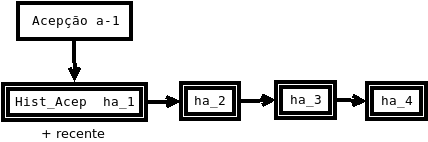
\includegraphics[width=.6\textwidth]{figuras/acep.png}
    \caption{Como estavam implementadas as acepções}
    \label{fig:acep}
\end{figure}

Mas havia um problema nessa implementação. O campo de ligação entre \kw{Acepção} e \kw{Histórico Acepção} só
ajuda a verificar o mais atual. Para descobrir o meis antigo (para achar o \emph{Terminus a quo} -- taq), é
necessário fazer de 0 a $n$ operações \texttt{JOIN} aumentando muito o custo da pesquisa por esta informação.
Trata-se de um potencial garagalo.

Antes de pensar nas mudanças, bom pensar a razão de se precisar das instâncias mais antiga e mais recente. A
importância da mais antiga se deve ao fato de que, através dela, pode-se conhecer a data aproximada ou real
da sua primeira aparição. A mais nova é importante pois através dela é que se determina a grafia atua da acepção.

Para refatorar a entidade, retirou-se o campo \texttt{:histacepatual\_id} da classe \kw{Acepção} e
\texttt{:anterior\_id} de \kw{Hist$\_$Acepção}. Além disso, criou-se uma referêcia da primeira na segunda classe,
e uma chave na classe de acepções para a mais antiga e mais recente. As mudanças na prática podem ser vistas na
tabela abaixo.

\begin{table}[h]
    \centering
    \begin{tabular}{|c|c|c|c|}
        \cline{3-4}
        \multicolumn{2}{c}{} & \multicolumn{2}{|c|}{Desempenho} \\ \hline
        operação & frequência & antes & depois \\ \hline
        acessar a mais recente & alta & \Oh{1}[1] & \Oh{1}[2] \\
        acessar a mais antiga & alta & \Oh{n}[3] & \Oh{1}[4] \\ \hline
        \multicolumn{4}{|c|}{Adicionando uma entrada em \kw{Hist$\_$Acepção}} \\ \hline
        atualizar mais recente & média-alta & \Oh{1}[5] & \Oh{1}[6] \\
        atualizar a mais antiga & média-alta & \Oh{n}[7] & \Oh{1}[8] \\ \hline
        \multicolumn{4}{|c|}{Removendo uma entrada em \kw{Hist$\_$Acepção}} \\ \hline
        atualizar mais recente & baixa & \Oh{1}[9] & \Oh{n*lg\ n}[10] \\
        atualizar a mais antiga & baixa & \Oh{n}[11] & \Oh{n*lg\ n}[12] \\ \hline
    \end{tabular}
    \caption{Comparativo do desempenho entre as versões antes e depois da refatoração \\
        Desempenho e frequêcia são estimados com base no fluxo conhecido de operação}
    \label{tab:comparing}
\end{table}

Justificativas:
\begin{itemize}
    \item Acessos
    \begin{description}
        \item[1, 2 e 4] Há uma chave que permite o acesso direto a essa instância
        \item[3] É necessário percorrer a lista inteira para encontrar a instâcia
    \end{description}
    \item Inserção
    \begin{description}
        \item[5, 6 e 8] Há uma chave que permite o acesso direto à instância a ser comparada
        \item[7] É necessário percorrer a lista para saber onde será colocado o próximo emelemnto
    \end{description}
    \item Remoção
    \begin{description}
        \item[9] Há uma chave que permite o acesso direto à instância a ser comparada, após a remoção,
        conecta-se o anterior à acepção
        \item[11] É necessário percorrer a lista inteira para chegar no último elemento, deletá-lo, e
        remover o seu registro do novo registro mais antigo
        \item[10 e 12] Após a remoção, pesquisa-se o elemento mais antigo ou recente. Isso depende da ordenação
        do histórico de acepções. Não se sabe em que algoritmo se baseia a ordenação do Ruby. Supondo que
        seja baseado em comapações, com certeza roda em \Oh{n*lg\ n}
    \end{description}
\end{itemize}

\paragraph{Porque tirar o nome e o taq da tabela de acepções?}

No \texttt{README.md} do projeto em Rails, sessão de perguntas, foi feita uma reflexão similar.\footnote{A
pergunta foi sobre a definição da acepção e da flexão} Nesta ocasião, a resposta foi \say{Depois de reflexões,
ficou claro que a definição pode ser alterada a cada inserção ou remoção de lemas. Gerar demanda de mais uma ou
duas pesquisas, ainda que simples, constitui um gargalo tolo, e por isso a definição de flexões ou acepções deve
ficar nas tabelas principais}. O erro principal desse raciocínio é o que uma ou duas pesquisas a mais provavelmente
não serão responsáveis por um gargalo tão grande assim. Além do mais, a implementação pode diminuir esse impacto.

Um outro fator a considerar é \href{https://pt.wikipedia.org/wiki/Lei_de_Demeter}{Lei de Demeter}. Segundo ela, é
importante que uma classe saiba muito pouco ou quase nada das outras classes. Utilizar Esse princípio não impediria
que se colocasse esses campos na tabela de acepções. Entretanto, ao implementar dessa forma, o projeto fica menos
acoplado, e portanto, mais flexível e menos difícil de escalar.

\paragraph{Nas operações de remoção de históricos de acepções o desempenho médio é pior considerando-se a solução
nova. Isso não pode ser um problema?}

Não, porque são operações que tiveram um desempenho estimado pior são as mesmas operações apontadas como
menos frequentes pelo cliente, enquanto as operações mais repetidas tiveram um melhoramento.

\subsection{N -- Por que a implementação do design pattern Builder foi abandonada na criação de formulários no front-end?}
\label{subsec:nuxt-left-design-pattern-builder}

A ideia inicial no que diz respeito aos formulários, é que haveria uma classe Javascript que geraria os formulários. Mas
por que fazer assim e não um formulário por vez?

O motivo é que fazer vários formulários pode resultar em repetição de código. Fazer isso não é pecado, mas reduz
a qualidade do código. Além do mais, código repetido pode requerer testes com mais código duplicado, reduzindo a ainda
mais a qualidade do código, sem mencionar a necessidade de se replicar determinadas mudanças.

Exite uma troca inerente no processo. Buscar um sistema mais enxuto e esclável implica, na maioria das ocasiões, em um
aumento (considerável ou não) de complexidade. Entretanto, uma vez implementado um construtor de formulários, pode-se
simplesmente chamar o componente com o tipo específico de formulário a se criar. Essa ideia veio de uma palestra sobre
como aplicar alguns design patterns no desenvolvimento com Vue.js. O vídeo desta palestra pode ser encontrado no YouTube
\footnote{O título do vídeo é \say{Phenomenal Design Patterns In Vue with Jacob Schatz}}, no site VueMastery, aba
Conference Videos \dir VueConf US 2019, e \href{https://read-and-watch.github.io/videos/RF1bbhRw9sg/index.html}{neste link}
se precisar de legendas para o vídeo.

\paragraph{Por que então os formulários não foram implementados desta forma então?} Ao tentar implememntar uma solução
similar, tive dificuldade, pois não sabia como passar os dados da requisição HTTP para o backend. Para evitar maiores
atrasos, decidi criar múltiplos componentes. Passado o prazo do TCC, é uma coisa que adoraria fazer com mais calma.

\subsection{N -- Existe uma quantidade considerável de código repetido no front. Isso não é algo ruim?}
\label{subsec:no-dry}

De fato. Em diversos momentos do desenvolvimento foi dito que repetir código era uma má prática, e não deixou de ser. O
problema, entretanto, foi conciliar a vontade de fazer a melhor aplicação, com o melhor cógigo, o mais limpo possível,
com a necessidade do DELPo de estar de pé. Não posso faltar com o respeito com os integrantes do NEHiLP, e entregar algo
que não funcione, mas também não posso escrever um código porco que a curto prazo nenhuma viva alma seria capaz de
compreender. Provavelmente é uma das coisas em que mais preciso amadurecer, e pude aprender um pouco mais com esse projeto.

\subsection{Por que não há testes feitos para o front end?}\label{subsec:no-tests-for-nuxt}

O motivo principal para não haver testes para o front é que o planejamento inicial previa aproveitar o conteúdo do curso
\href{https://vueschool.io/courses/learn-how-to-test-vuejs-components}{\say{Testing Vue.js Components}} fazendo os testes
para a aplicação do front. Como eu desconheço quaisquer outras ferramentas de teste para Javascript, e o Jest é muito
parecido com o RSpec, e eu tinha um curso bem estruturado (os cursos desta plataforma são muito bons), decidi optar por
ela, memso correndo o risco de ficar sem esses testes de front.

\section{A aplicação está pronta? Como isso impacta os resultados esperados?}
\label{sec:is-it-ready}

Não. A aplicação não está completa em nenhum dos dois lados. Ela está funcional, mas falta juntar essas peças que foram
verificadas.

No back end, tudo o que estava funcionando  na versão anterior, continua funcionando nesta também. A diferença é a
qualidade do código, e algumas otimizações, sem contar na melhor organização do projeto. Aliás, adiantando uma das
reflexões na sessão \ref{sec:lessions}, aprendi um pouco com esse projeto como balancear o ímpeto de fazer um código
seguindo design patterns e um código que fique pronto em tempo hábil. Houveram múltiplas ocasiões em que se perderam dias,
semanas ou ainda mais tempo pensando em como fazer determinada funcionalidade da melhor forma ao invés de simplesmente
fazer acontecer.

Se por um lado, o desenvolvimento ocorreu num ritmo reduzido, por outro, o código resultante apresenta uma qualidade
formidável:
\begin{itemize}
    \item grande encapsulamento entre classes
    \item pouquíssimo código repetido (concentrados na parte do front e nos testes do Rails)
    \item extensa cobertura de testes (não tive tempo de testar os componentes do front)
    \item as dependências entre componentes não engessam a aplicação
\end{itemize}

Obviamente trata-se de uma escolha entre qualidade e agilidade; qualidade versus quantidade. Optou-se pela primeira em
nome do comprometimento com o cliente que apresenta uma grande necessidade de ver sua aplicação a funcionar sem maiores
problemas como acontece atualmente.

Outra coisa a se observar quanto ao desenvolvimento Rails é observar que nada se perdeu apesar da grande reconstrução
feita. O controlador do moedor ainda não foi implementado ainda, mas todo o arcabouço funcional por trás disso está.
Como verificar isso? Simples. Tudo funcionava antes da grande refatoração, então basta levar em conta o que se passa com
cada parte do código. O que foi modificado agora funciona sem sombra de dúvida, e da mesma maneira (dado que o que foi
mudado foi a forma de fazer o código e não o que este fazia). O que não foi alterado ainda se encaixa com o resto do
código pois nada foi modificado ali em termos de funcionamento.

Um grande avanço observado foi na interface. Ela estava muito crua no início do ano, e agora ela apresenta um grande
dinamismo. Ainda que o seu desenvolvimento esteja na fase de construção do sistema de admissibilidade de usuários, e da
gestão de tokens, e pareça \say{cru}, é claro que não há muito o que deixar para o próximo desenvolvedor\footnote{Ainda
que eu pretenda continuar a fazer o projeto mesmo depois de concluido o TCC.}.

Respondendo a última parte da pergunta, com certeza não vou receber um 10 por este trabalho. No entanto, se se levar
em conta o balanço do que foi feito e do que não foi, perceber-se-á que o saldo foi extremamente positivo. Veja abaixo.

\begin{table}[h]
    \centering
    \begin{tabular}{|c|c|c|}
        \hline
        \multicolumn{3}{|c|}{Atividades} \\ \hline\hline
        Concluidas & Não Concluídas & Não iniciadas \\ \hline
        Refatorar o banco dedados & Fazer um interface de  & Adaptação dos dados \\
        & usuário agradável (60\%) & da aplicação antiga \\ \hline
        Refatoração dos modelos  & Fazer os testes no back (73\%) & Fazer os testes do front \\
        e controladores & & \\ \hline
        Modularização das classes  & & \\
        e interfaces  & & \\ \hline\hline
        \multicolumn{3}{|c|}{\textbf{Observações}} \\ \hline
        \multicolumn{3}{|c|}{As porcentagens na coluna do meio são uma estimativa do grau de conclusão da tarefa} \\ \hline
    \end{tabular}
    \caption{Tarefas do projeto}
    \label{table:activity}
\end{table}